% ==============================================================================
% TCC - César Henrique Bernabé
% Capítulo 3 - Zanshin e Unagi
% Falar sobre os problemas do modelo antigo do zanshin
% Falar sobre novo metamodelo e explicar como cheguei nele
% Falar o prq do novo metamodelo ser melhor que o anterior e quais as novidades
% Falar sobre as vantagens do novo metamodelo no arquivo XML
% Falar das restricoes inseridas no novo metamodelo
% Falar dos problemas do novo metamodelo
% Falar de refinamentos (OR, AND, só pode ser AND ou OR, etc) e que agora quase todos os requisitos possuem refinamentos
% ==============================================================================

\chapter{Zanshin}
\label{sec-zanshin}

Esta seção trata do processo de reavaliação do metamodelo operacional do sistema \zanshin, anteriormente já apresentado na Figura~\ref{figura-metamodelo-antigo}.

\section{Motivação}
\label{sec-zanshin-motivacao}
Durante estudos realizados sobre a implementação do \framework \zanshin, detectaram-se algumas oportunidades de melhoria relacionadas principalmente ao metamodelo de objetivos utilizado pelo sistema. A maioria das oportunidades de melhoria identificadas referem-se a dois motivos: ou o metamodelo não era restrito o suficiente, deixando que algumas situações indesejadas pudessem ser modeladas; ou o metamodelo não refletia mais alguns conceitos de \gore que foram melhores elaborados em discussões recentes sobre o tema. 


\section{Revisão do Metamodelo}
\label{sec-zanshin-revisao}
Uma análise de cada elemento do metamodelo antigo é feita a seguir:

\begin{enumerate}
	%1
	\item \textbf{Requirement}: o fato desse elemento estar no topo da hierarquia e todos os outros elementos serem especializações dele faz com que suas características sejam herdadas por todos os outros componentes do modelo. Porém, nota-se que algumas características na verdade são inerentes a apenas alguns elementos. Por exemplo: \textit{Requirement} possui a relação de agregação \textit{Parent} para \textit{Children}, permitindo que cada elemento tenha zero ou um ``Pai'' e um ou vários ``Filhos''. Entretanto, a agregação pai/filho é indesejada nos elementos \awreq, \textit{DomainAssumption} e \textit{QualityConstraint}, visto que esses não são refinados, apenas possuem elementos alvo.
	
	%2
	\item \textbf{DeinableRequirement} e \textbf{Softgoal}: \sofgoal possui o mesmo tipo de comportamento de um \textit{DefinableRequirement} e portanto, seria esperado que aquele também fosse uma especialização deste. Assim, com essa modificação faz-se-ia desnecessário a utilização de duas classes (\textit{Requirement} e \textit{DefinableRequirement}) na composição do modelo, que poderiam perfeitamente ser reduzidas a apenas uma.
	
	%3
	\item \textbf{Softgoal} e \textbf{QualityConstraint}: baseando-se no fato de que \textit{Softgoals} são compostos de \textit{Quallity Constraints} pode-se identificar que a relação mais apropriada a esses dois elementos seria a relação de composição. Além disso, o modelo permite que um \textit{Softgoal} contenha nenhuma operacionalização, o que não faria sentido pois assim não seria possível identificar quando esse elemento foi bem sucedido ou não.
	
	%4
	\item \textbf{DefinableRequirement} e \textbf{AwReq}: de acordo com as propostas apresentadas na literatura atual para os \awreqs, fica claro que esses elementos, ao se referirem a qualquer outro tipo de elemento e tratarem especificamente do elemento ao qual se referem, deveriam ter na verdade uma relação de composição com o elemento mais alto da hierarquia de especializações, permitindo então que todos os outros elementos do modelo contessem \awreqs.
	
	%5
	\item \textbf{Goal} e \textbf{Task}: \textit{Tasks} são refinamentos de \textit{Goal} e por isso seria importante que houvesse algum tipo de relacão direta entre os dois elementos, onde fosse possível identificar que quando um objetivo fosse operacionalizado por tarefas e quais seriam essas tarefas. Além disso, identificou-se uma oportunidade de melhoria da nomenclatura de ``\textit{Goal}'' para ``\textit{HardGoal}'', refletindo assim uma melhor impressão sobre o papel do elemento e a diferença entre ele e \sofgoal.
	
	%6
	\item \textbf{DomainAssumption}: não é claro no modelo a forma como \textit{DomainAssumptions} se relacionam com os outros elementos.
\end{enumerate}

\section{Proposta}
\label{sec-zanshin-proposta}

Após levantamento das melhorias possíveis, foi elaborado o metamodelo apresentado na Figura~\ref{figura-metamodelo-novo}. 

\begin{figure}[h]
	\centering
	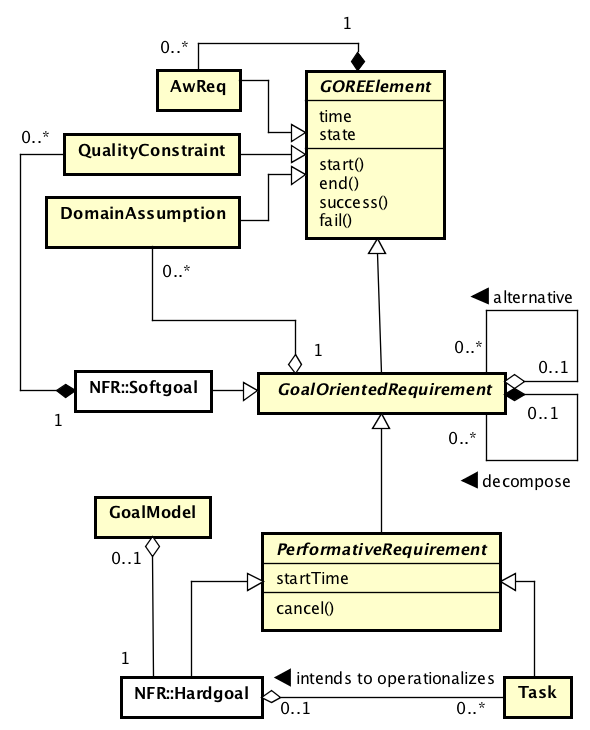
\includegraphics[width=0.7\textwidth]{figuras/metamodelos/metamodelo-zanshin-novo.png}
	\caption{Proposta de evolução do metamodelo do \framework \zanshin}
	\label{figura-metamodelo-novo}
\end{figure}

Primeiramente, pode-se observar que o as especialiações e relações de agregação e composição entre os elementos foram refinadas, assim, identifica-se que:

\begin{itemize}
	\item A partir de agora, todos os elementos são especializações de \textit{GOREElement}, que passa a englobar características das antigas classes \textit{Requirement} e \textit{DefinableRequirement}, resolvendo então parte do problema [2]. 

	\item A agregação pai/filho agora ocorre em dois tipos e acontece em um elemento mais específico: um requisito pode ser decomposto (\textit{decompose}) em outros, referindo-se assim a refinamentos do tipo ``E'', ou refinado através da agregação denominada ``alternative'', que trata de alternativas a um requisito, ou seja, refinamentos do tipo ``OU''. Dessa forma o metamodelo pode retratar melhor os tipos de refinamentos admitidos e quais são, exatamente, os componentes que  os aceitam. Além do mais, a partir desta melhoria os refinamentos acontecem somente nos elementos que especializam \textit{GoalOrientedRequirement}, ou seja, somente \textit{Hardgoals}, \textit{Softgoal} e \textit{Tasks}. Essa modificação soluciona o problema [1].

	\item Nessa nova proposta, há uma relação de decomposição entre o elemento raiz (\textit{GOREElement}) e \awreq, portanto, explicita-se a noção de que qualquer requisito pode conter requisitos adaptativos, eliminando a outra parte do problema [2]. Isso também tem um efeito positivo em relação a especificação do \xml usado para criar modelos específicos de domínio, que fica mais claro e conciso.
	
	\item \textit{Softgoal} e \textit{QualityConstraint} passam a se relacionar por meio de relação de decomposição, e portanto também fica mais evidente que todo \textit{Softgoal} deve ser operacionalizado por pelo menos um \textit{QualityConstraint}, dando fim assim ao problema [3].
	
	\item Nessa proposta, \awreqs tem uma relação direta de composição com o \textit{GOREElement}, e portanto, define-se que qualquer tipo de requisito no modelo pode conter elementos de adaptação, assim resolve-se o problema [4].
	
	\item No novo metamodelo, foi criada uma relação direta entre \textit{Tasks} e \textit{Hardgoals} (previamente apenas \textit{Goals}), assim fica explícito o relacionamento entre esses dois elementos, sinalizando que objetivos são refinados em tarefas, que podem ser refinadas apenas nelas mesmas. Soluciona-se então o problema [5].
	
	\item Propõe-se, por fim, uma relação de agregação entre \textit{DomainAssumption} e \textit{GoalOrientedRequirement}, assim fica claro que \textit{Domain Assumptions} são elementos que interagem apenas com Objetivos e Tarefas (\textit{Hardgoals}, \textit{Softgoal} e \textit{Tasks}), findando o problema [6].
	
\end{itemize}

Uma observação importante que deve ser feita refere-se ao fato de que um elemento só pode conter refinamentos exclusivamente do tipo ``E'' (``AND'') ou exclusivamente do tipo ``OR''. Essa decisão tem por objetivo facilitar a leitura e interpretação do diagrama, e não compromete a representatividade do modelo pois assume-se que se necessário, pode-se agrupar refinamentos do mesmo tipo em um objetivo, como exemplificado na Figura~\ref{figura-refinamentos}.

\begin{figure}[h]
	\centering
	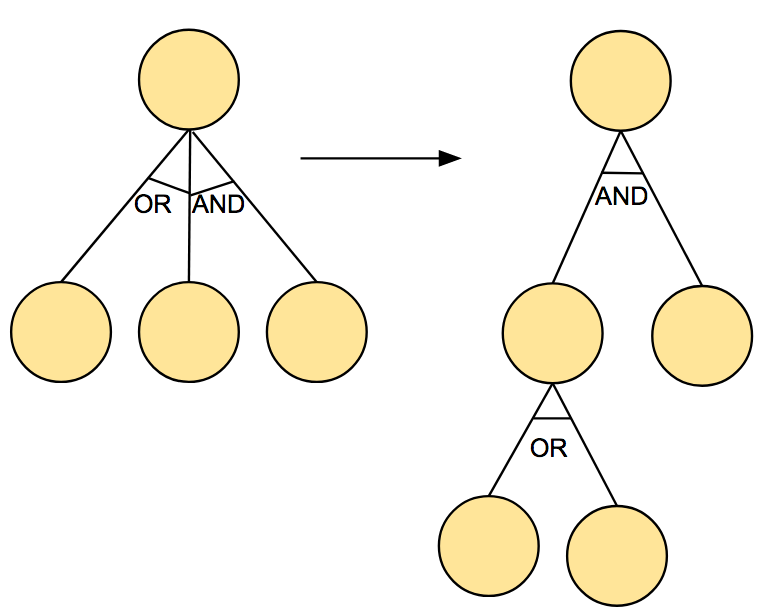
\includegraphics[width=0.7\textwidth]{figuras/metamodelos/exemplo-or-and.png}
	\caption{Exemplificação da representação de refinamentos no novo metamodelo.}
	\label{figura-refinamentos}
\end{figure}